\documentclass[compress]{beamer}
\usepackage{themesimple} % load sty file
\usefonttheme{professionalfonts}

% other packages
\usepackage[brazilian]{babel}
\usepackage[utf8]{inputenc}
\usepackage[T1]{fontenc}
\usepackage{lmodern}
\usepackage[scale=2]{ccicons}
\usepackage{xcolor}
\usepackage{pgfplots}
\pgfplotsset{compat=newest}

%\usepackage[table]{xcolor}
%\usepackage{graphics}
%\usepackage{multirow}
%\usepackage{multicol}
%\usepackage{adjustbox} % for \adjincludegraphics
%\usepackage{etoolbox}
%\usepackage[absolute,overlay]{textpos}
%\usepackage{fancybox}
%\usepackage{ctable}
%\usepackage{changepage}


\definecolor{hughesblue}{rgb}{.9,.9,1} 





\renewcommand\lstlistingname{R}% Change language of section name

\lstset{ % General setup for the package
	language=R,
	keepspaces=true, % keeps spaces in text
	basicstyle=\small\sffamily,
	numbers=left,
 	numberstyle=\tiny,
 	frame=tb,
	tabsize=4,
	columns=fixed,
	showstringspaces=false,
	showtabs=false,
	keepspaces,
	commentstyle=\color{red},
	keywordstyle=\color{blue}
}


\AtBeginSection[]{%
  \begin{frame}
  \vfill
  \centering
  \begin{beamercolorbox}[sep=8pt,center,shadow=true,rounded=true]{title}
    \usebeamerfont{title}\secname\par%
  \end{beamercolorbox}
  \vfill
  \end{frame}
}%




% changing rounded bullets and their color in the table of contents
\setbeamerfont{section number projected}{size=\small}
\setbeamercolor{section number projected}{bg=darkgray,fg=white}
\setbeamertemplate{sections/subsections in toc}[circle] %ball, circle, square


% Printing the Handout
% \usepackage{pgfpages}
% \pgfpagelayout{resize}[a4paper,border shrink=5mm,landscape]
% This says resize all pages to landscape A4 pages, no what their original size was, but shrink the pages by 5mm, so that there is a bit of a border around everything. \pgfpagelayout{2 on 1}[a4paper,border shrink=5mm]

\setbeamertemplate{blocks}[rounded][shadow=true]

\newcommand{\backupbegin}{%
   \newcounter{framenumberappendix}
   \setcounter{framenumberappendix}{\value{framenumber}}
}%
\newcommand{\backupend}{%
   \addtocounter{framenumberappendix}{-\value{framenumber}}
   \addtocounter{framenumber}{\value{framenumberappendix}}
}%

\setbeamercovered{invisible}

\pgfplotsset{compat=1.11}

\title{Perfil das Comunidades Terapêuticas no Brasil}
%\subtitle{}
\date{Junho 07, 2016}
\author{Maria Paula \\ Daniel Marcelino \\ Luiz Philipe Reis \\
Nayara Villar \\ Vinnie Nasser \\ Marcello Lira Doudement
}
\institute{Instituto de Pesquisa Econômica Aplicada}

\logo{%
  \makebox[0.99\paperwidth]{%
    \hfill%
    
\includegraphics[width=1cm,keepaspectratio]{figures/logo-ipea.png}%
  }%
}

\begin{document}
%\SweaveOpts{concordance=TRUE}
%\Sweave2knitr{concordance=TRUE}



%-------------------------------------
\begin{frame}
\maketitle
\end{frame}
%-------------------------------------



%-------------------------------------
\begin{frame}{Apresentação}
\tableofcontents
\end{frame}
%-------------------------------------



%-------------------------------------
\section{Introdução}
\begin{frame}{Introdução}

\begin{exampleblock}{}
\begin{itemize}[<+-| alert@+>]
	\item Pesquisa realizada pelo IPEA, através da DIEST, por encomenda da Secretaria Nacional de Política de Drogas (SENAD/Ministério da Justiça), e financiada com recursos repassados por esta mesma secretaria ao IPEA.
	\item Comunidades Terapêuticas (CTs): entidades da sociedade civil que têm por objetivo apoiar pessoas que fazem uso problemático de substâncias psicoativas (SPAs).
	\item Se constituem como residências coletivas, muitas delas situadas em áreas rurais, em que os indivíduos devem ingressar voluntariamente, e ali permanecer até que alcancem condições físicas e psíquicas para prosseguirem em suas trajetórias de vida, sem o uso de drogas.
	\item Princípios: abstinência; recuperação pela fé e pelo trabalho.
\end{itemize}
\end{exampleblock}
\end{frame}
%-------------------------------------


%-------------------------------------
\begin{frame}[plain]
\begin{figure}[h]
\centering
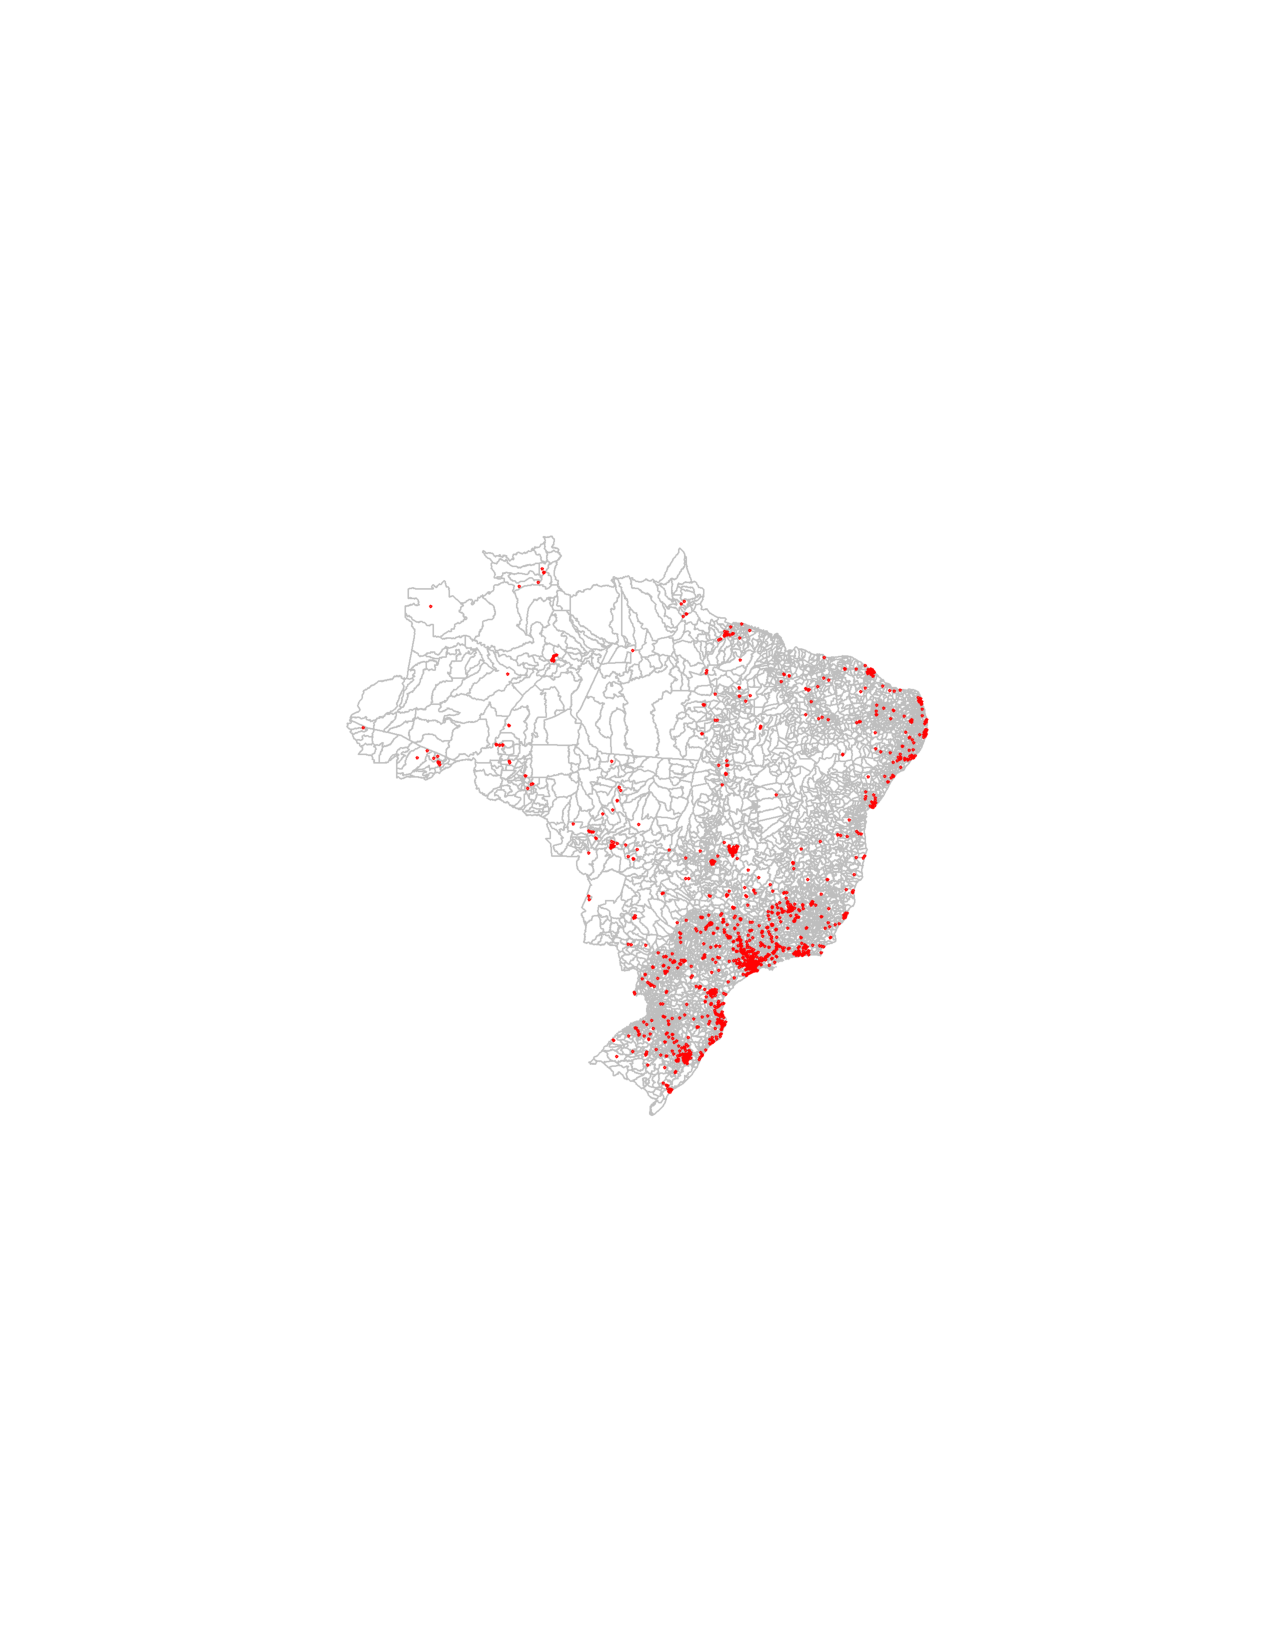
\includegraphics[height=.85\textheight, keepaspectratio]{figures/mapa.pdf}
\caption{Distribuição geográfica da população de CTs, considerando o cadastro disponível}
\label{fig:distrCTs}
\end{figure}
\end{frame}
%-------------------------------------


%-------------------------------------
\section{Metodologia}
\begin{frame}{Metodologia}

A pesquisa proposta previa duas estratégias: {\bf quantitativa} e {\bf qualitativa}

\begin{block}{}

\begin{itemize}
	\item {\bf Quantitativa:} survey junto a um amplo conjunto de CTs, situadas nas diversas regiões do país.
	\item {\bf Qualitativa:} trabalho de campo intensivo, etnográfico, para conhecimento em profundidade das práticas das Comunidades Terapêuticas: suas rotinas, as relações que estabelecem com seus acolhidos; relações com as redes do SUS e do SUAS.
\end{itemize}

\end{block}{}

\end{frame}
%-------------------------------------


%-------------------------------------
\subsection{Survey}
\begin{frame}{Survey}


\begin{block}{Informações pretendidas:}
	
\begin{itemize}
	\item porte das diversas CTs;
	\item a magnitude da oferta de vagas;
	\item os segmentos etários, e por gênero, da população acolhida;
	\item a orientação religiosa das entidades;
	\item seus recursos financeiros;
	\item o tamanho e a composição suas instalações;
	\item suas regras de convivência;
	\item suas relações com outros serviços de cuidado, especialmente aqueles de Saúde e de Assistência Social; entre outros
\end{itemize}

\end{block}

\end{frame}
%-------------------------------------

%-------------------------------------
\begin{frame}{Survey}


\begin{block}{Informações pretendidas:}
	
\begin{itemize}
	\item Possível a partir da localização e captura, na Internet, de um cadastro com 1863 CTs, situadas em todo o Brasil.
	\item Embora de autoria incerta, traz informações relevantes: nome das CTs, telefone, e-mail e coordenadas de localização.
	\item Estas permitem o acesso às entidades, assim como a extração de uma amostra delas, para fins do survey.
	\end{itemize}

\end{block}

\end{frame}
%-------------------------------------


%-------------------------------------
\begin{frame}{Survey}


\begin{block}{Informações pretendidas:}
	
\begin{itemize}
	\item Aplicação dos questionários: feita por meio da Internet, em software livre, adaptado pela TI do Ipea às necessidades da pesquisa e disponibilizado em plataforma.
	\item CTs receberam um formulário eletrônico, acessével através de um link, enviado por e-mail.
	\item Questionário preenchido na própria plataforma. As respostas ingressam imediatamente na base de dados, de onde são exportadas como planilhas, a partir das quais são tabuladas e analisadas.
\end{itemize}

\end{block}

\end{frame}
%-------------------------------------


%-------------------------------------
\section{Desenho Amostral}

\begin{frame}{Redes Urbanas}


\begin{block}{}
\begin{itemize}
	\item Conceito de rede urbana: conjuntos de cidades que se conectam em função da oferta de bens e serviços.
	\item Algumas cidades (em geral, as maiores) são lugares de produção e distribuição de bens e serviços, enquanto outras (normalmente, as menores) recorrem aos bens e serviços produzidos e distribuídos nas primeiras.
	\item Estas conexões se traduziriam em hierarquias entre cidades: algumas cidades se tornam mais importantes que outras, em virtude dos fluxos que atraem, em busca de sua oferta de bens e serviços
	
\end{itemize}
\end{block}

	


\end{frame}
%-------------------------------------


%-------------------------------------
\begin{frame}{REGICS no Brasil}
Desde os anos 60, o IBGE realiza estudos com o objetivo de conhecer estes fluxos e os relacionamentos entre as cidades brasileiras, definindo as Regiões de Influência das Cidades (REGIC).


\begin{block}{Estes estudos buscam:}
[...] definir a hierarquia dos centros urbanos e delimitar as regiões de influência a eles associadas a partir dos aspectos de gestão federal e empresarial e da dotação de equipamentos e serviços, de modo a identificar os pontos do território a partir dos quais são emitidas decisões e é exercido o comando em uma rede de cidades (IBGE:2007).
\end{block}

	


\end{frame}
%-------------------------------------

%-------------------------------------
\begin{frame}{REGICS no Brasil}
{Na atualização de 2007 (IBGE), as cidades brasileiras foram classificadas em cinco grandes níveis, a saber:}


\begin{itemize}
\item Metrópoles, representadas pelos 12 principais centros urbanos do país;
\item Capitais regionais, constituídas 70 grandes cidades que têm área de influência
de âmbito regional;
\item Centros sub-regionais, compostos por 169 cidades com atividades de gestão menos complexas;
\item Centros de zona, formados por 556 cidades de menor porte e com atuação restrita à sua área imediata; e
\item Centros locais, representados pelas demais 4.473 cidades cuja centralidade e atuação não extrapolam os limites do seu município, servindo apenas aos seus habitantes.
\end{itemize}
	


\end{frame}
%-------------------------------------

%-------------------------------------
\begin{frame}{Adaptação da Classificação REGIC}

\begin{block}{Estratificação:}
	Para a estratificação da amostra das CTs, segundo o porte e a importância das cidades nas quais se situam, foram utilizadas as classificações da REGIC 2007, aglutinadas em apenas três estratos, de modo a reduzir o número de estratos considerados.
\end{block}




\begin{block}{Os três estratos adotados foram então:}
\begin{itemize}
\item Estrato Metrópole/Capital Regional--que aglutina os estratos 1 e 2 da classificação original;
\item Estrato Centro Sub-regional, que coincide com o estrato 3, de classificação original; e
\item Estrato Centro Local/Centro de Zona--no qual foram reunidos os estratos 4 e 5 da
classificação acima.
\end{itemize}
	
\end{block}
\end{frame}
%-------------------------------------


%-------------------------------------
\begin{frame}{Desenho Amostral}

\begin{itemize}
	\item A amostra é obtida por amostragem estratificada simples, tendo por objetivo estimar proporções para a população de CTs das informações de interesse, controladas pela localização geográfica dessas unidades.
	\item Os estratos naturais são especificados a partir do cruzamento da macrorregião e da categoria REGIC em que está localizada a CT.
	\item Os estratos finais são definidos de acordo com a condição e financiamento pela SENAD. O estrato final certo (com probabilidade de seleção igual a 1) é formado pelas CTs que recebem financiamento da Secretaria; o estrato final amostrado é formado pelas CTs presentes no cadastro, mas que não são financiadas pela Secretaria. Dessa forma, a amostra é estratificada da seguinte maneira.
	
\end{itemize}



\end{frame}
%-------------------------------------



%-------------------------------------
\begin{frame}{Desenho Amostral}
\centering
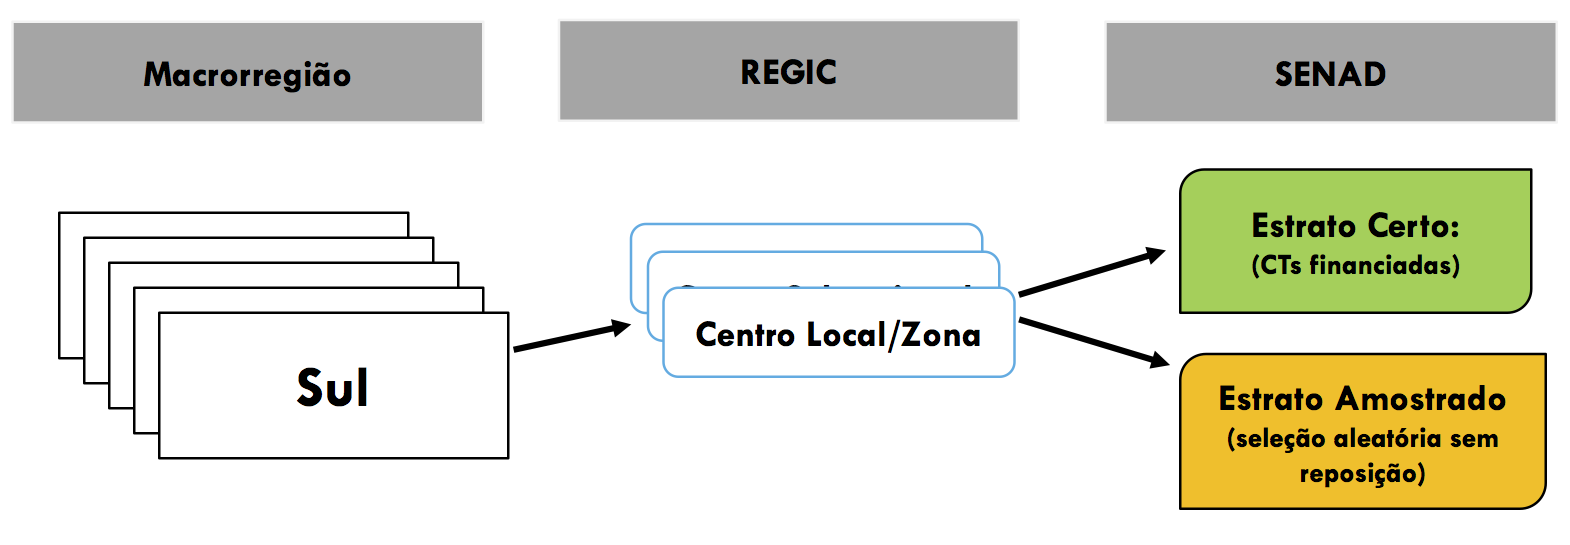
\includegraphics[width=1\textwidth, keepaspectratio]{figures/desenho.png}
\end{frame}
%-------------------------------------



%-------------------------------------


\begin{frame}{Another title}
    Some text\\
    \uncover<2->{Uncover me on slide 2 (-)\\}
    \visible<3->{visible from slide 3 on (-)\\}
    \only<4->{only from slide 4 (-)\\}
    \onslide<5->{on slide 5 and further (-)\\}
    \uncover<6>{Uncover me on slide 6 \\}
    \visible<7>{visible on 7\\}
    \only<8>{only on slide 8 \\}
    \alt<8>{I am on slide 8\\}{I am not on slide 8\\}
    \onslide<9>{on slide 9\\}
\end{frame}
%-------------------------------------




\begin{frame}
\frametitle{Rigid body dynamics}

\tikzstyle{na} = [baseline=-.5ex]

\begin{itemize}[<+-| alert@+>]
    \item Coriolis acceleration
        \tikz[na] \node[coordinate] (n1) {};
\end{itemize}

% Below we mix an ordinary equation with TikZ nodes. Note that we have to
% adjust the baseline of the nodes to get proper alignment with the rest of
% the equation.
\begin{equation*}
\vec{a}_p = \vec{a}_o+\frac{{}^bd^2}{dt^2}\vec{r} +
        \tikz[baseline]{
            \node[fill=blue!20,anchor=base] (t1)
            {$ 2\vec{\omega}_{ib}\times\frac{{}^bd}{dt}\vec{r}$};
        } +
        \tikz[baseline]{
            \node[fill=red!20, ellipse,anchor=base] (t2)
            {$\vec{\alpha}_{ib}\times\vec{r}$};
        } +
        \tikz[baseline]{
            \node[fill=green!20,anchor=base] (t3)
            {$\vec{\omega}_{ib}\times(\vec{\omega}_{ib}\times\vec{r})$};
        }
\end{equation*}

\begin{itemize}[<+-| alert@+>]
    \item Transversal acceleration
        \tikz[na]\node [coordinate] (n2) {};
    \item Centripetal acceleration
        \tikz[na]\node [coordinate] (n3) {};
\end{itemize}

% Now it's time to draw some edges between the global nodes. Note that we
% have to apply the 'overlay' style.
\begin{tikzpicture}[overlay]
        \path[->]<1-> (n1) edge [bend left] (t1);
        \path[->]<2-> (n2) edge [bend right] (t2);
        \path[->]<3-> (n3) edge [out=0, in=-90] (t3);
\end{tikzpicture}
\end{frame}


%-------------------------------------
\begin{frame}{Alguns Resultados}
\centering
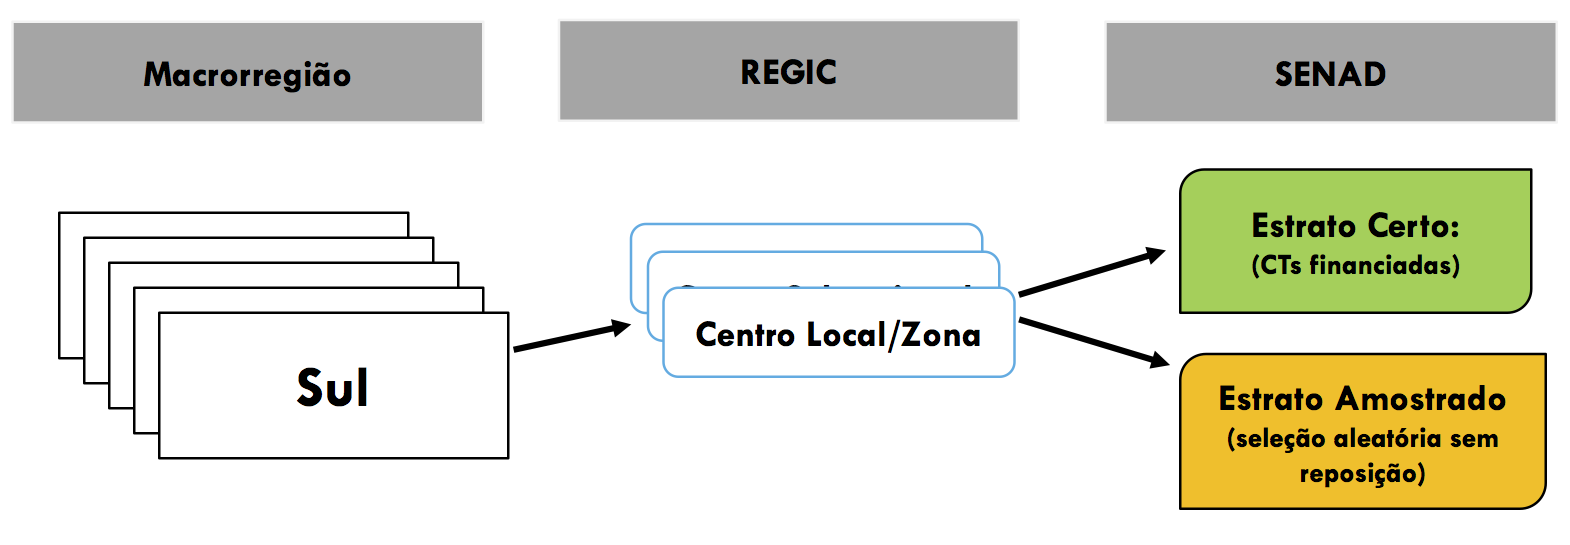
\includegraphics[width=1\textwidth, keepaspectratio]{figures/desenho.png}
\end{frame}
%-------------------------------------


%-------------------------------------
\begin{frame}{Alguns Resultados}


\end{frame}
%-------------------------------------



\appendix

\backupbegin

\begin{frame}[plain]
Proudly created with \LaTeXe
\end{frame}
\backupend



\end{document}

